\chapter{序論}
我々の身の回りにある物質を構成する最小単位は素粒子である。
物質の最小単位である素粒子と、素粒子の相互作用を記述した理論として標準模型が存在している。素粒子物理学において、自然界には電磁相互作用、強い相互作用、弱い相互作用、重力相互作用といった4種類の基本相互作用が存在すると考えられており、標準模型では重力相互作用以外の3種類の相互作用が記述されている。
標準模型は図\ref{fig:標準模型}に示すように、12種類のフェルミオン、4種類のゲージボソン、ヒッグス粒子の計17種類の粒子から構成されており、2012年に唯一実験的に未確認であったヒッグス粒子が発見された\cite{article:Higgs_boson}。
\begin{figure}[tb]
  \centering
  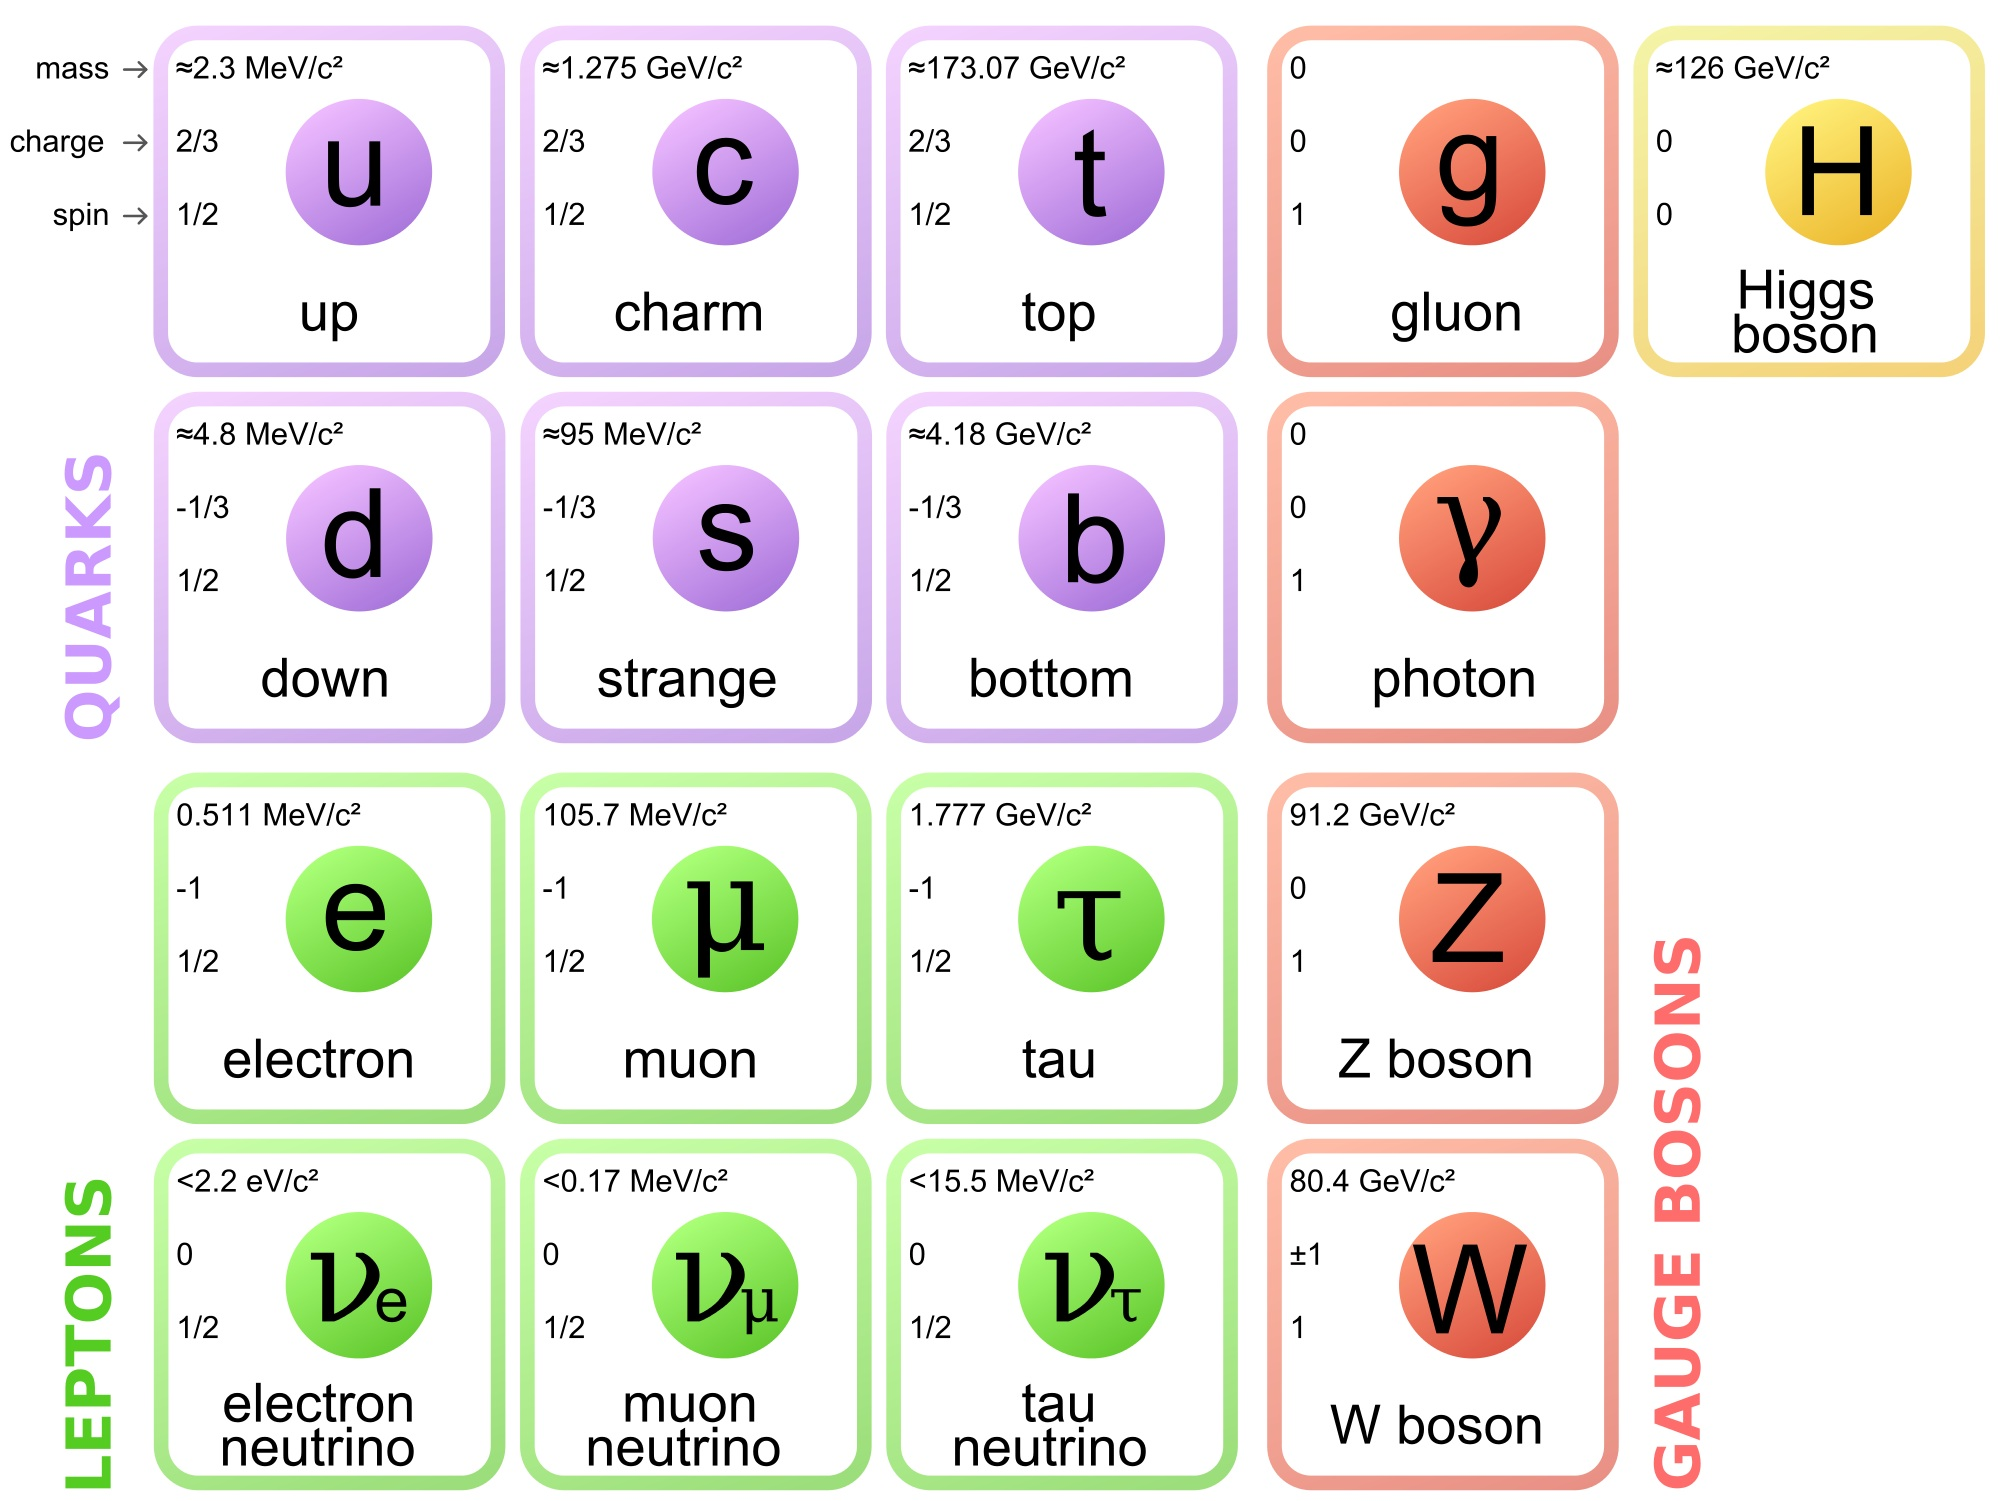
\includegraphics[clip, width=10cm]{fig/1/standardmodel.jpg}
  \caption{標準模型を構成する17種類の素粒子\cite{article:elementary_particles}。}
  \label{fig:標準模型}
\end{figure}

現在、標準模型は多くの物理事象を説明することができているが、ダークマターの存在や階層問題などの多くの未解決問題が残されている。
この問題を解決するためには、標準模型を超える新しい物理が必要であり、この新物理を探索するために世界中で様々なアプローチの実験が行われている。

このアプローチの一つとして、ジュネーブ郊外に位置する欧州原子核研究機構 (CERN) の地下に設置された Large Hadron Collider (LHC) を用いる高エネルギーの陽子陽子衝突実験がある。LHC を使った衝突実験の1つである ATLAS 実験では、ATLAS 検出器と呼ばれる大型汎用検出器を用いて陽子-陽子衝突によって生成される粒子を検出し、TeV スケールの物理事象までの測定を行い標準理論を構成する素粒子の精密測定や超対称性粒子の探索を目的としている。

ATLAS 実験では陽子を$40$ MHzの頻度で衝突させたデータを用いて新物理探索を行っている。しかし、計算機リソースやデータ容量などの観点からこの高頻度での陽子-陽子衝突事象を全て保存することができない。そのため、トリガーシステムを使った事象選別を行うことで膨大な量のデータから物理として興味のある事象を選別し、保存可能なデータ量まで事象を減らして保存している。
ATLAS 検出器では、1段目にはハードウェアベースの高速処理が可能な初段トリガー (Level-1 Trigger)、2段目ではソフトウェアベースで精密処理が可能な後段トリガー (High-Level Trigger) のような2段階のトリガーシステムが実装されている。

本研究では、この初段トリガー、特にミューオンをターゲットにして事象選別を行う初段エンドキャプ部ミューオントリガーに着目する。
ATLAS 検出器の最外層に位置するミューオン検出器には、衝突点からのミューオンのみが飛来するため粒子の同定が容易であり、短時間でトリガーを発行することができる。さらに、ヒッグス粒子の崩壊先である Z ボソンや W ボソンの終状態として高い運動量のミューオンが観測されやすいことや、ボトムクォークやチャームクォークが含まれる粒子の終状態には運動量が低いミューオンが含まれる。そのためミューオンは 陽子-陽子衝突実験において様々な物理事象のサインとして重宝されている。

LHC 及び ATLAS 検出器は 2018 年から 2021 年までの期間にアップグレードが行われ、2022 年から Run-3 として運転が再開された。アップグレードを行ったことで、Run-3 では陽子-陽子衝突の重心系エネルギーの増強や最高瞬間ルミノシティでの安定した運転に伴い、背景事象による事象頻度 (トリガーレート) が増加する。したがって、限られた記憶容量の中で物理事象を最大効率で取得するために、初段トリガーにおいてもトリガーシステムの改良を行い、トリガーレートを抑えつつ、トリガー判定の精度を維持・向上させる必要がある。

本論文では、ミューオンをターゲットにして事象選別を行う初段エンドキャプ部ミューオントリガーに対する改良を行い性能評価について述べる。






